\begin{frame}{Informações do desenvolvimento}
	\begin{columns}
		\column{0.4\textwidth}
		\begin{minipage}[c][0.4\textheight][c]{\linewidth}
			\centering
			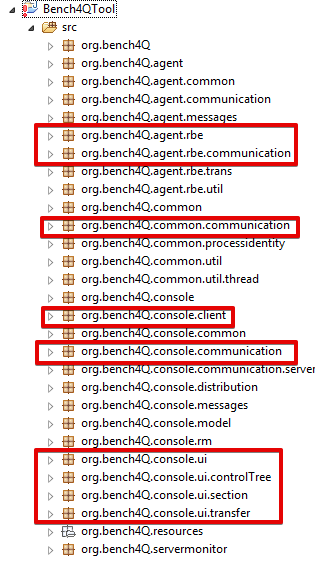
\includegraphics[scale=0.45]{images/project-bench4Q2.png}
		\end{minipage}
		\column{0.6\textwidth}
		\begin{minipage}[c][0.4\textheight][c]{\linewidth}
			\begin{itemize}
				\item O projeto original do Bench4Q é codificado em Java
				\begin{itemize}
					\item contêm 473 classes Java, com 46.029 linhas de código
					\item A extensão impacta todos os módulos, exceto o SUT
				\end{itemize}
				\item Extensão foi feita no IDE Eclipse
				\item A versão do Java utilizado foi a 1.6
				\item O código fonte está disponível em \footnote{\href{URL}{http://gitlab.lasdpc.icmc.usp.br/edwin/bench4q}}
			\end{itemize}
		\end{minipage}		
	\end{columns}
	
\end{frame}

\begin{frame}{Classes adicionadas e modificadas pela extensão}
	\begin{figure}[htb]
		\centering
		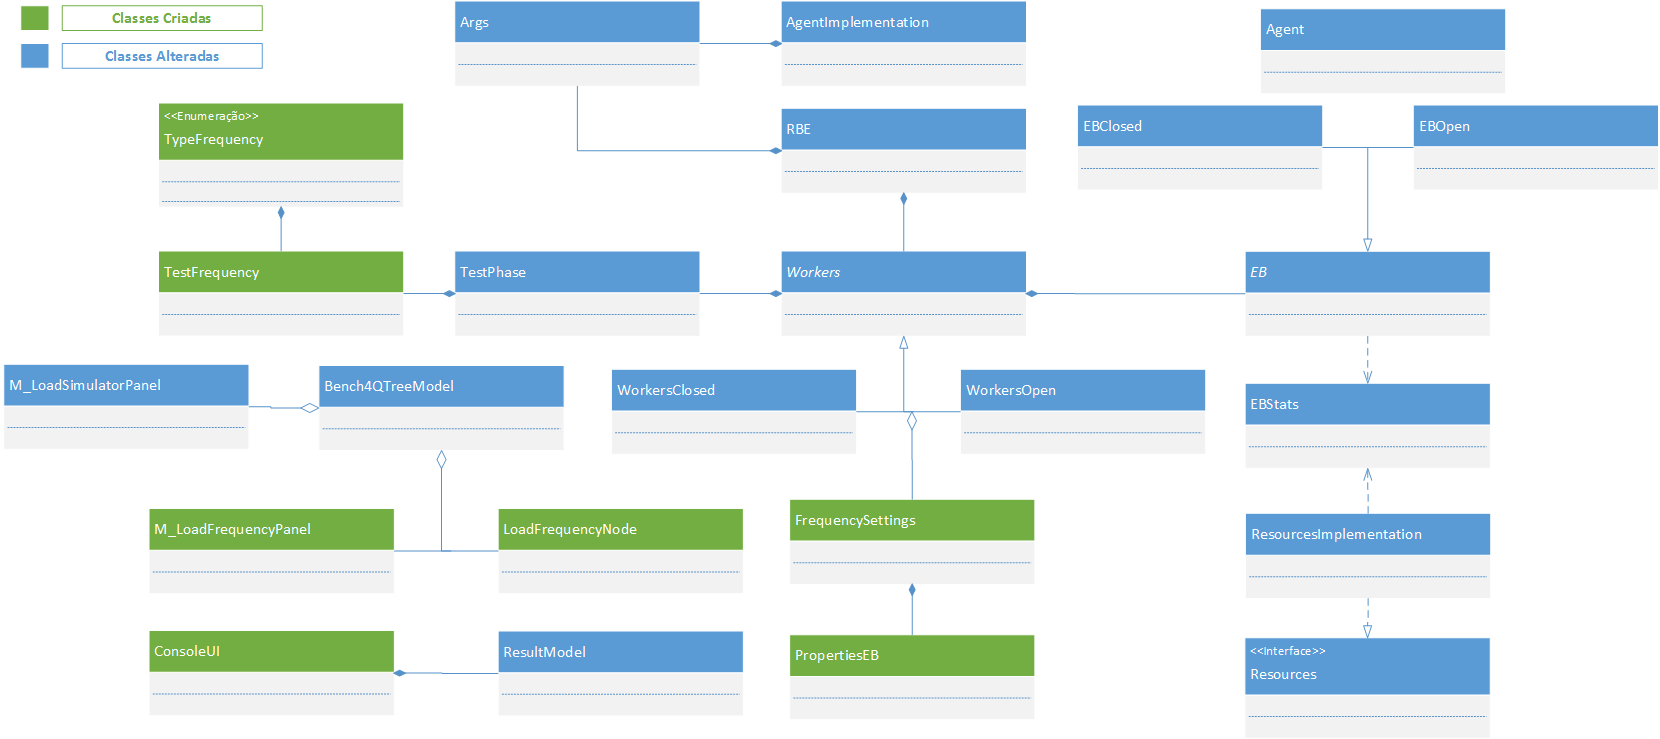
\includegraphics[scale=0.3]{../monograph/images/diagrama-classes-beanch4Q.png}	
	\end{figure}
\end{frame}

\begin{frame}{Implementação da carga de trabalho}
	\begin{figure}
		\centering
		\begin{minipage}{.3\textwidth}
			\centering
			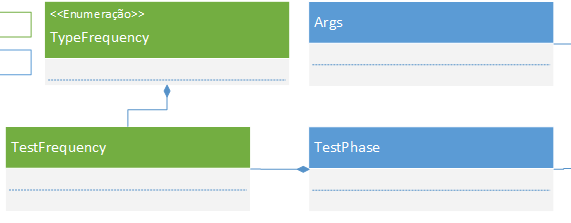
\includegraphics[scale=0.23]{images/diagram-code1.png}	
		\end{minipage}
		\begin{minipage}{.6\textwidth}
			\centering
			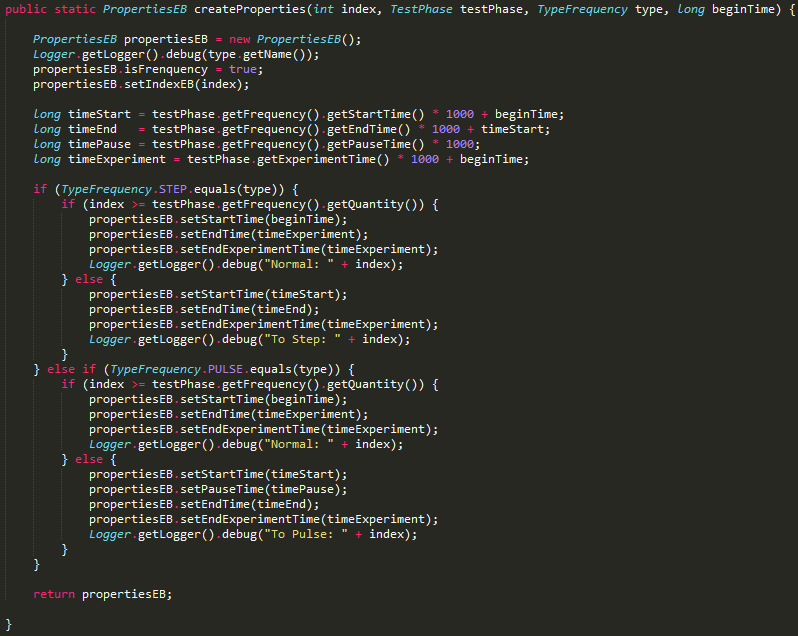
\includegraphics[scale=0.35]{images/code1.png} 
			%\caption{A subfigure}
		\end{minipage}
		\caption{Classe criada para a extensão}
	\end{figure}
	
\end{frame}

\begin{frame}{Implementação da carga de trabalho}
	\begin{figure}[htb]
		\centering
		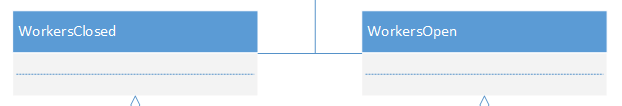
\includegraphics[scale=0.38]{images/diagram-code2.png}	
	\end{figure}
	\begin{figure}
		\centering
		\begin{minipage}{.45\textwidth}
			\centering
			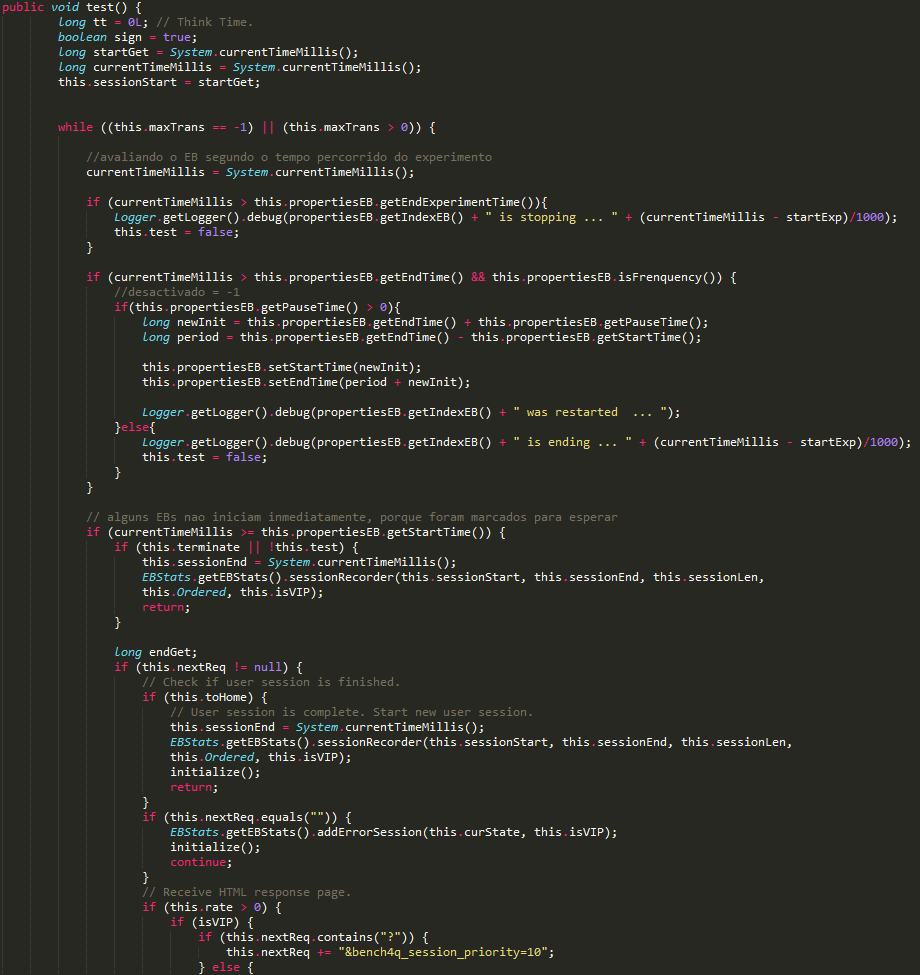
\includegraphics[scale=0.2]{images/code2-1.png}	
			%\caption{A subfigure}
		\end{minipage}
		\begin{minipage}{.45\textwidth}
			\centering
			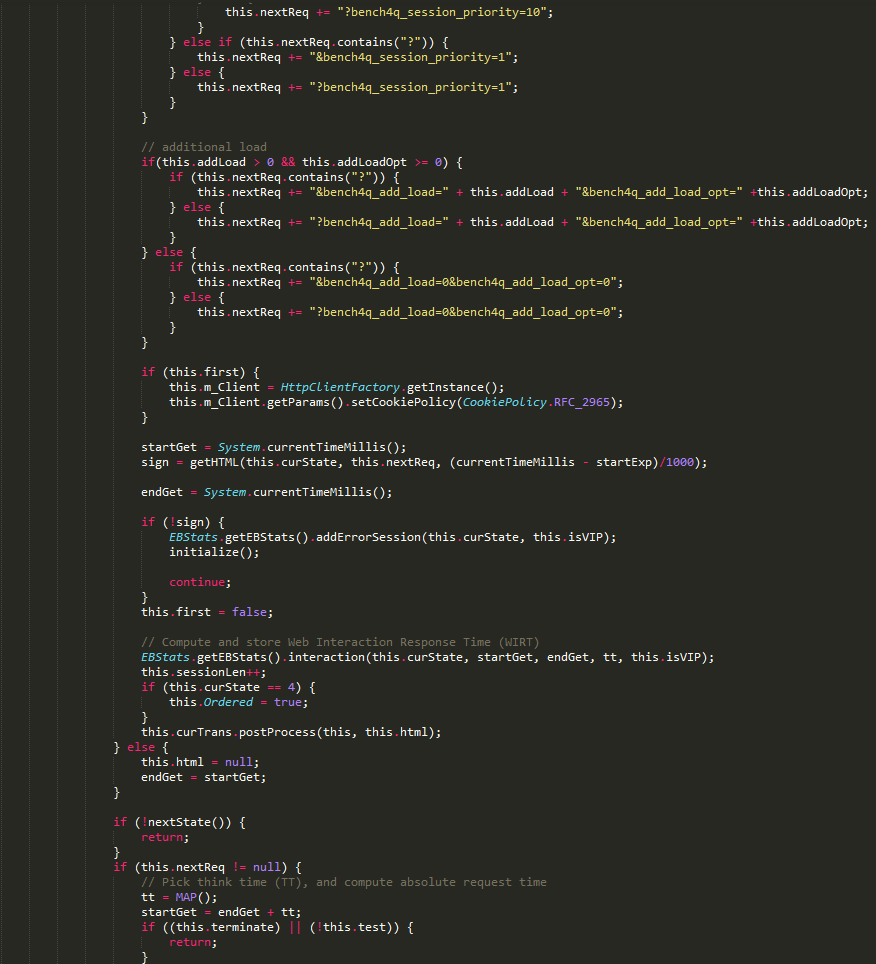
\includegraphics[scale=0.2]{images/code2-2.png}	
			%\caption{A subfigure}
		\end{minipage}
		\caption{Alteração em um método nativo do \textit{benchmark}}
	\end{figure}
	
\end{frame}

\begin{frame}{Implementação da carga de trabalho}
	\begin{figure}
		\centering
		\begin{minipage}{.3\textwidth}
			\centering
			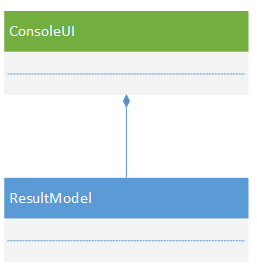
\includegraphics[scale=0.35]{images/diagram-code3.png}	
			%\caption{A subfigure}
		\end{minipage}
		\begin{minipage}{.6\textwidth}
			\centering
			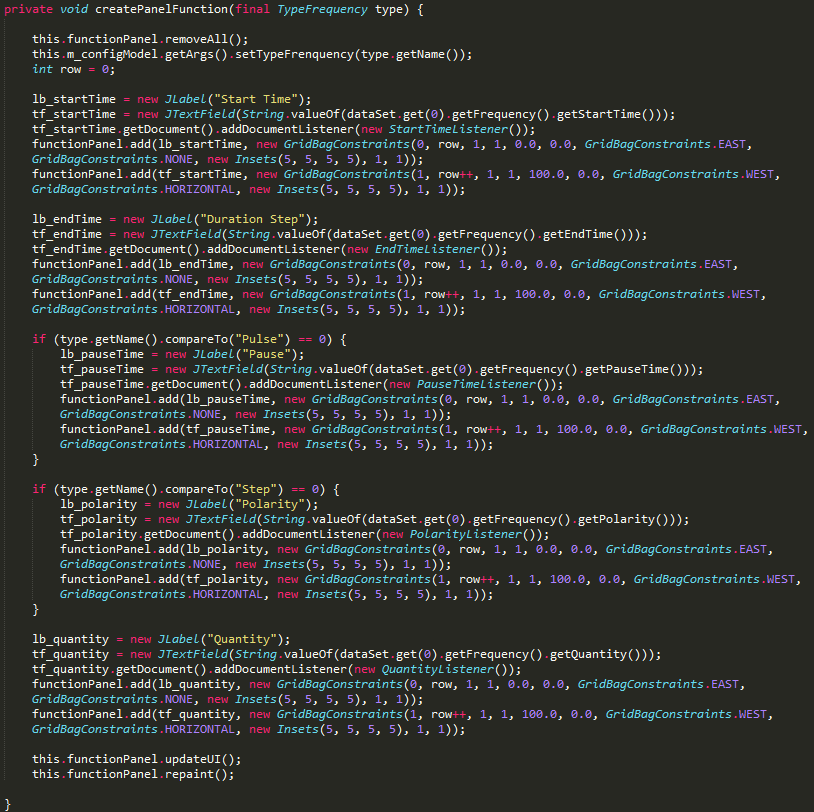
\includegraphics[scale=0.3]{images/code3.png}	
			%\caption{A subfigure}
		\end{minipage}
		\caption{Método de criação da interface gráfica para a modulação da carga}
	\end{figure}
	
\end{frame}


\begin{frame}{Teste de modulação}
	\begin{figure}[!htb]
		\centering
		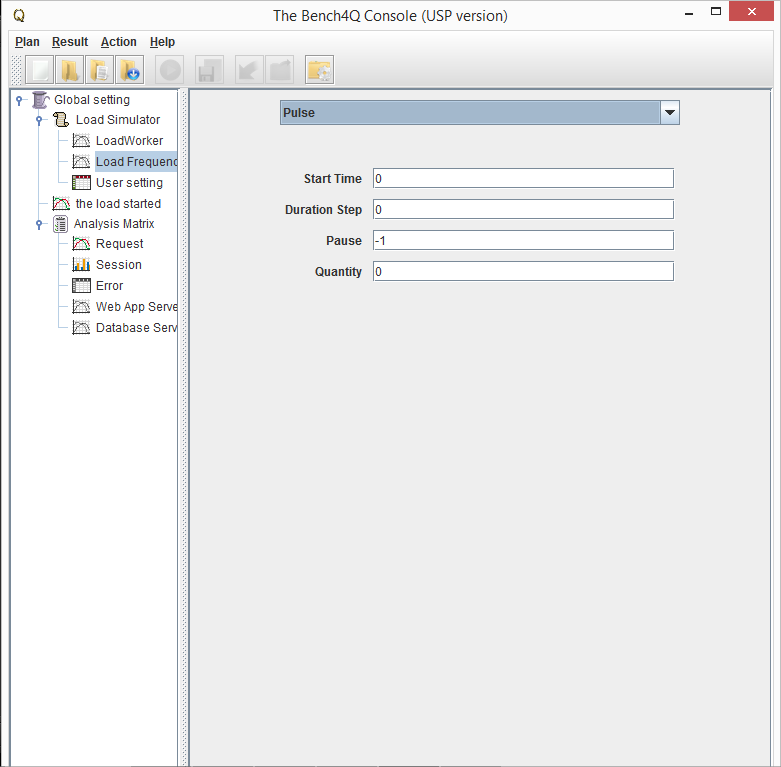
\includegraphics[scale=0.3]{../monograph/images/console-bench4Q-usp.png}
		\caption{Console de programação da carga de trabalho.}
		\label{fig:interface-criada-beanch4q}
	\end{figure}
\end{frame}

\begin{frame}{Teste de implementação}
	\begin{figure}
		\centering
		\begin{minipage}{.35\textwidth}
			\centering
			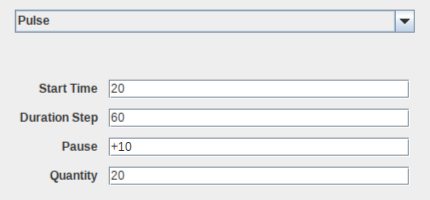
\includegraphics[scale=0.37]{../monograph/images/condiguracao-carga-modulada1.png}
		\end{minipage}
		\begin{minipage}{.45\textwidth}
			\centering
			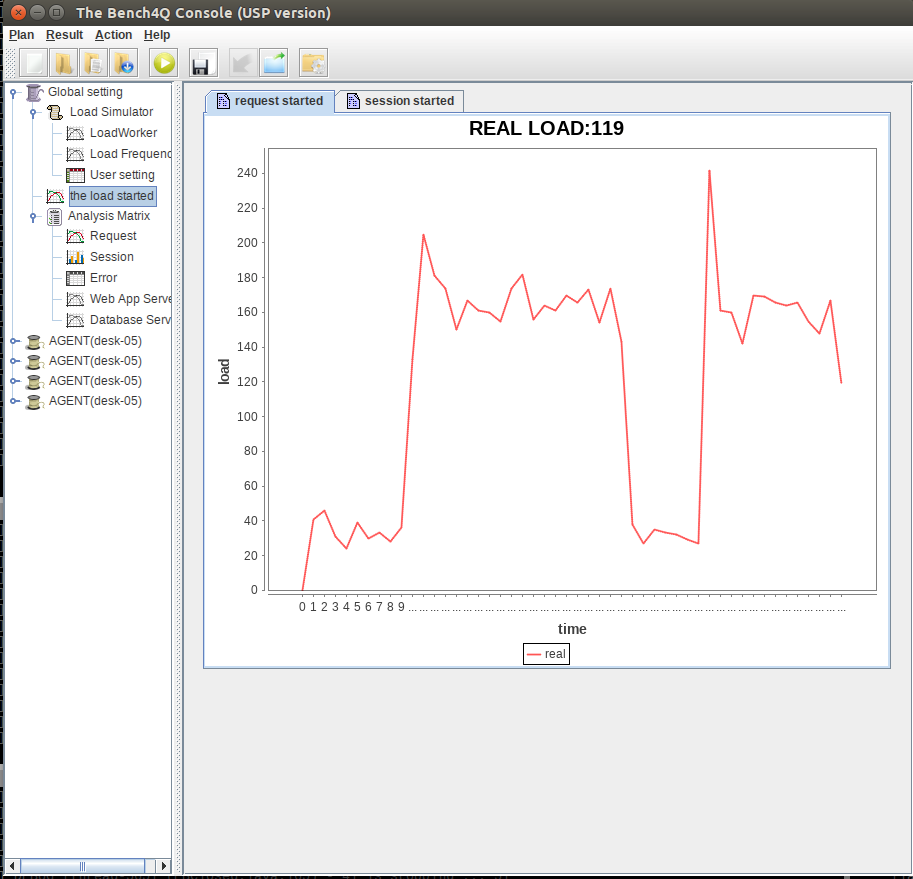
\includegraphics[scale=0.27]{../monograph/images/grafico-carga-modulada-teste.png}			
		\end{minipage}
		\caption{ensaios realizados para verificação da modulação}
	\end{figure}
\end{frame}



